\chapter{Свободное движение}
Рассмотрим систему 2-го порядка, заданную дифференциальным уравнением:
\[
\ddot y + a_1 \dot y + a_0 y = u
\]

Перепишем уравнение в операторной форме:
\[
p^2 y + a_1 p y + a_0 y = u
\]
\[
y = \frac{1}{p}\left(\frac{1}{p}(u - a_0 y) - a_1 y\right)
\]

Создадим Simulink модель по полученному уравнению:
\begin{figure}[H]
    \centering
    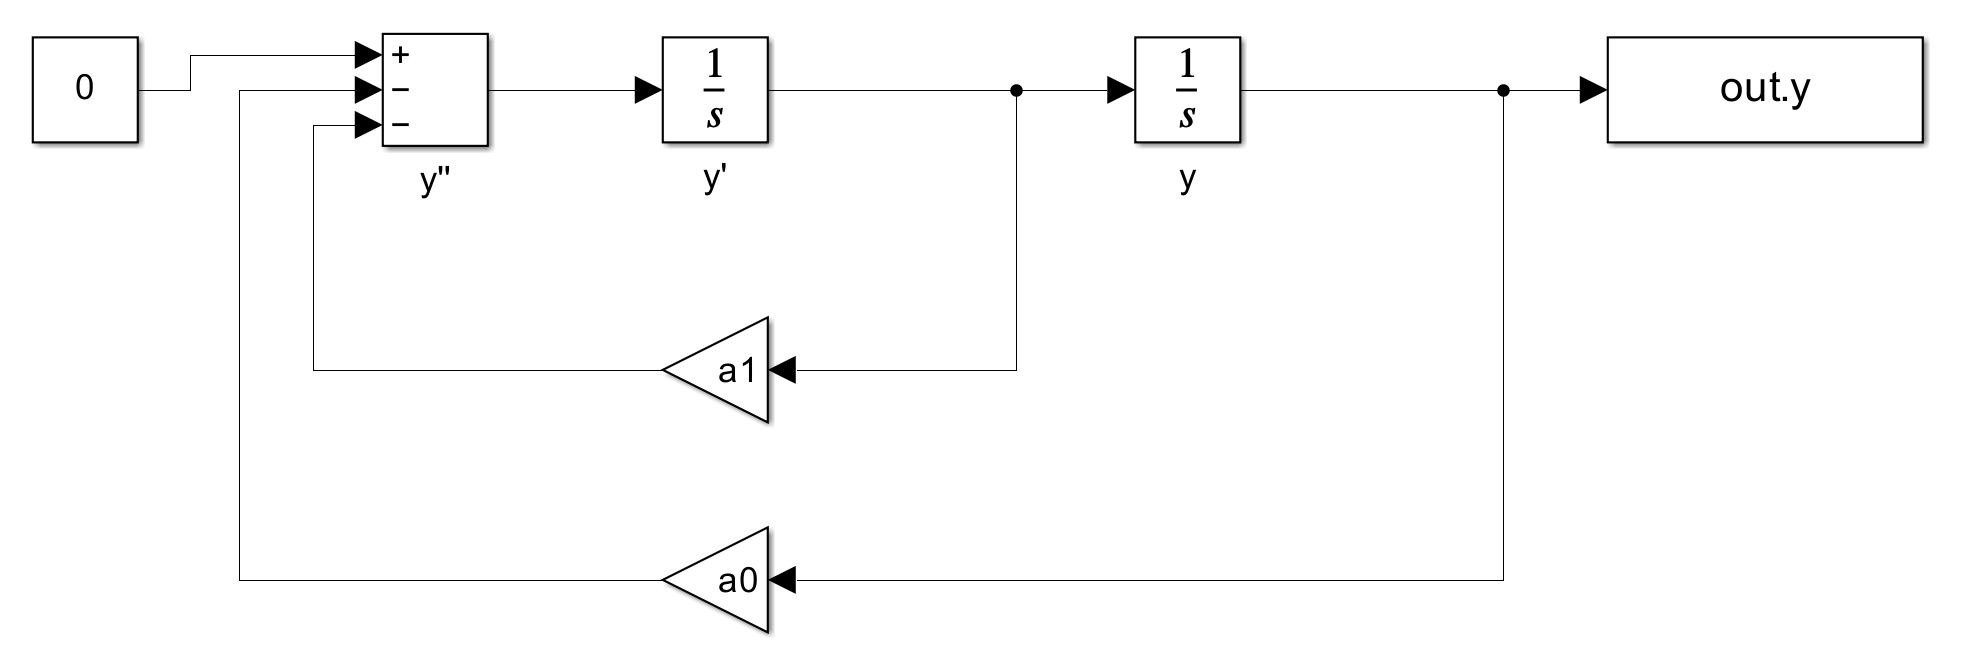
\includegraphics[width=1\textwidth, trim={0cm 0cm 0cm 0cm}]{../images/sim1.png}
    \caption{Схема Simulink}
    \label{fig:sim1}
\end{figure}

Теперь для каждого из 6 экспериментов найдем коэффициенты $a_0$, $a_1$ и аналитическое выражение свободной составляющей движения $y_{\text{св}}(t)$.
\section{Эксперимент 1}
\[y(0) = 1,\, \dot y(0) = 0 \quad \lambda_1 = -3,\, \lambda_2 = -1\]

По характеристическим корням построим исходное уравнение:
\[(\lambda - \lambda_1)(\lambda - \lambda_2) = (\lambda + 3)(\lambda + 1) = \lambda^2 + 4\lambda + 3 = 0\]

Отсюда $a_0 = 3$, $a_1 = 4$. Теперь по характеристическим корням найдем выражение свободной составляющей движения в общем виде:
\[y_{\text{св}}(t) = C_1 e^{\lambda_1 t} + C_2 e^{\lambda_2 t}\]

Найдем производную:
\[\dot y_{\text{св}}(t) = C_1 \lambda_1 e^{\lambda_1 t} + C_2 \lambda_2 e^{\lambda_2 t}\]

Подставим начальные условия:
\[y_{\text{св}}(0) = C_1 + C_2 = 1\]
\[\dot y_{\text{св}}(0) = -3\,C_1 -1\,C_2 = 0\]
\[C_1 = -\frac{1}{2},\, C_2 = \frac{3}{2}\]

\[y_{\text{св}}(t) = -\frac{1}{2}e^{-3t} + \frac{3}{2}e^{-t}\]

Сравним результаты моделирования и аналитического решения:
\begin{figure}[H]
    \centering
    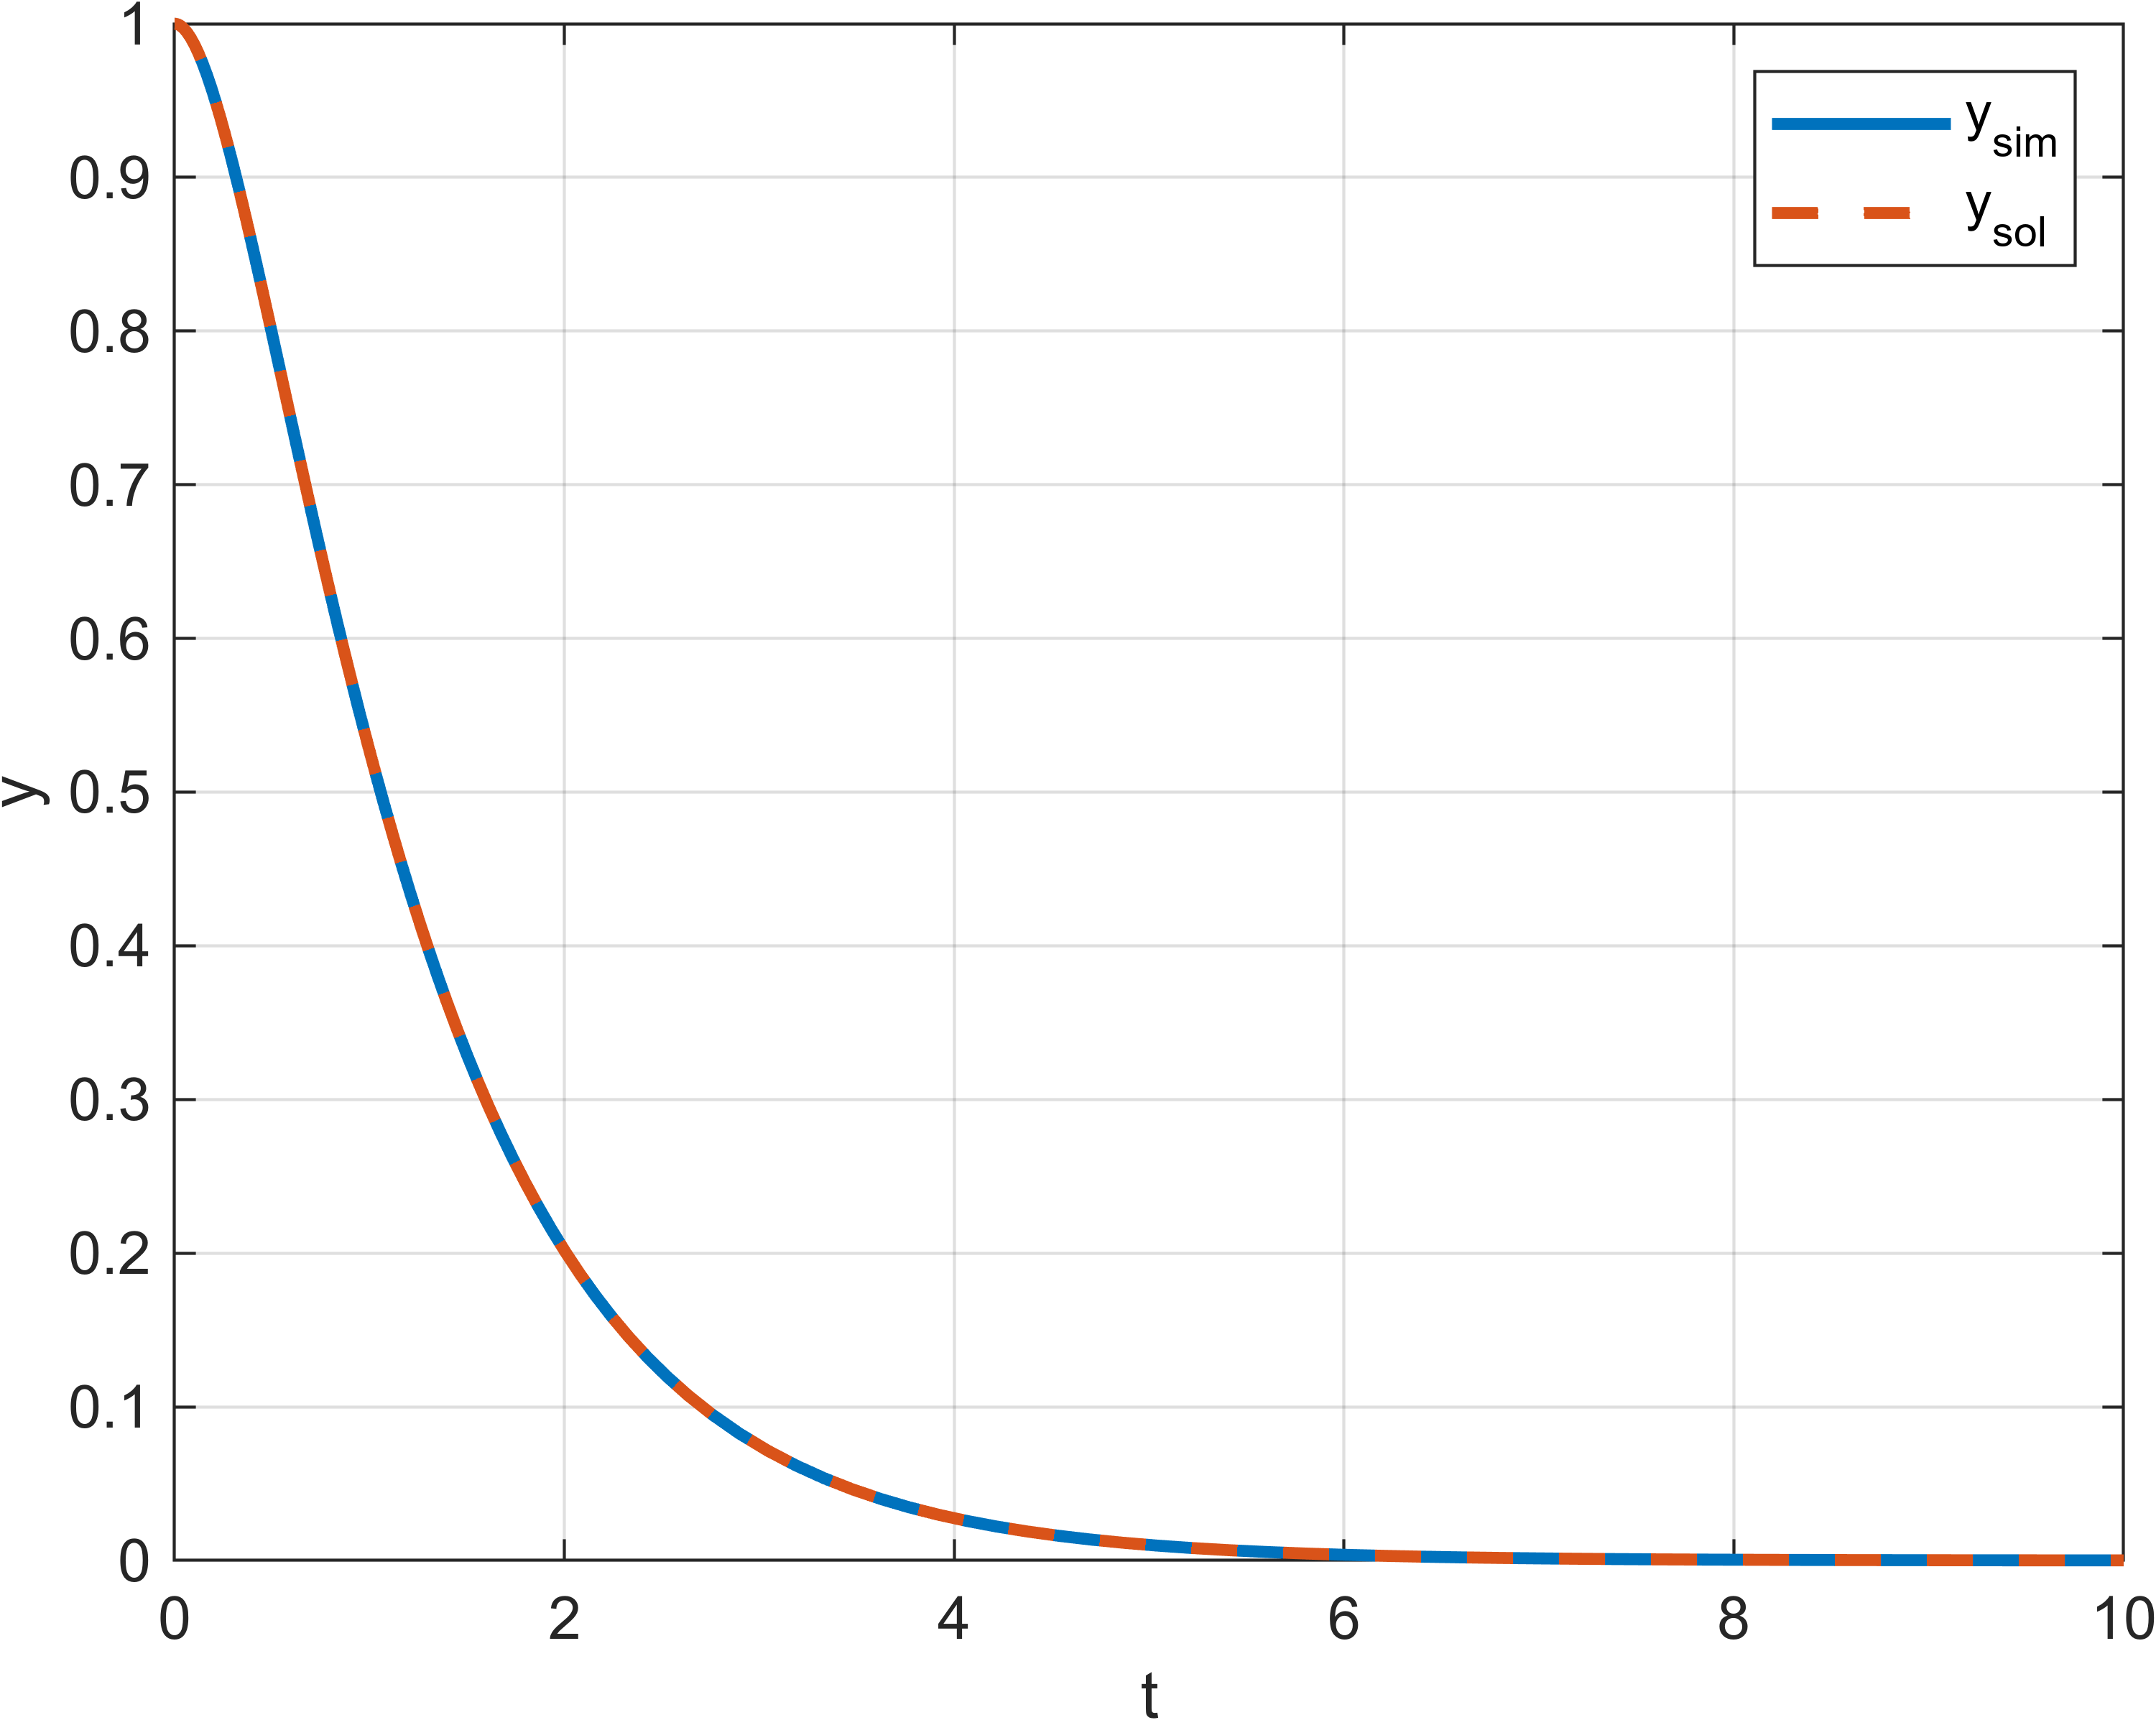
\includegraphics[width=1\textwidth, trim={0cm 0cm 0cm 0cm}]{../images/1_1.png}
    \caption{Эксперимент 1}
    \label{fig:exp1}
\end{figure}

Графики совпадают. Значит, аналитическое решение верно. Также можно заметить, что система асимптотически устойчива, так как все корни имеют отрицательные вещественные части.
\section{Эксперимент 2}
\[y(0) = 1,\, \dot y(0) = 0 \quad \lambda_1 = -1.1 + j9,\, \lambda_2 = -1.1 - j9\]

Также как и в прошлом эксперименте по характеристическим корням построим исходное уравнение:
\[(\lambda - \lambda_1)(\lambda - \lambda_2) = (\lambda + 1.1 - j9)(\lambda + 1.1 + j9) = \lambda^2 + 2.2\lambda + 82.21 = 0\]

Отсюда $a_0 = 82.21$, $a_1 = 2.2$. Теперь по характеристическим корням найдем выражение свободной составляющей движения в общем виде:
\[y_{\text{св}}(t) = C_1 e^{-1.1 t} sin(9t) + C_2 e^{-1.1 t} cos(9t)\]

Найдем производную:
\[\dot y_{\text{св}}(t) = -1.1C_1 e^{-1.1 t} sin(9t) + 9C_1 e^{-1.1 t} cos(9t) - 1.1C_2 e^{-1.1 t} cos(9t) - 9C_2 e^{-1.1 t} sin(9t)\]

Подставим начальные условия:
\[y_{\text{св}}(0) = C_2 = 1\]
\[\dot y_{\text{св}}(0) =  9C_1 - 1.1C_2 = 0\]
\[C_1 = \frac{1.1}{9}\]

\[y_{\text{св}}(t) = \frac{1.1}{9} e^{-1.1 t} sin(9t) + e^{-1.1 t} cos(9t)\]

Сравним результаты моделирования и аналитического решения:
\begin{figure}[H]
    \centering
    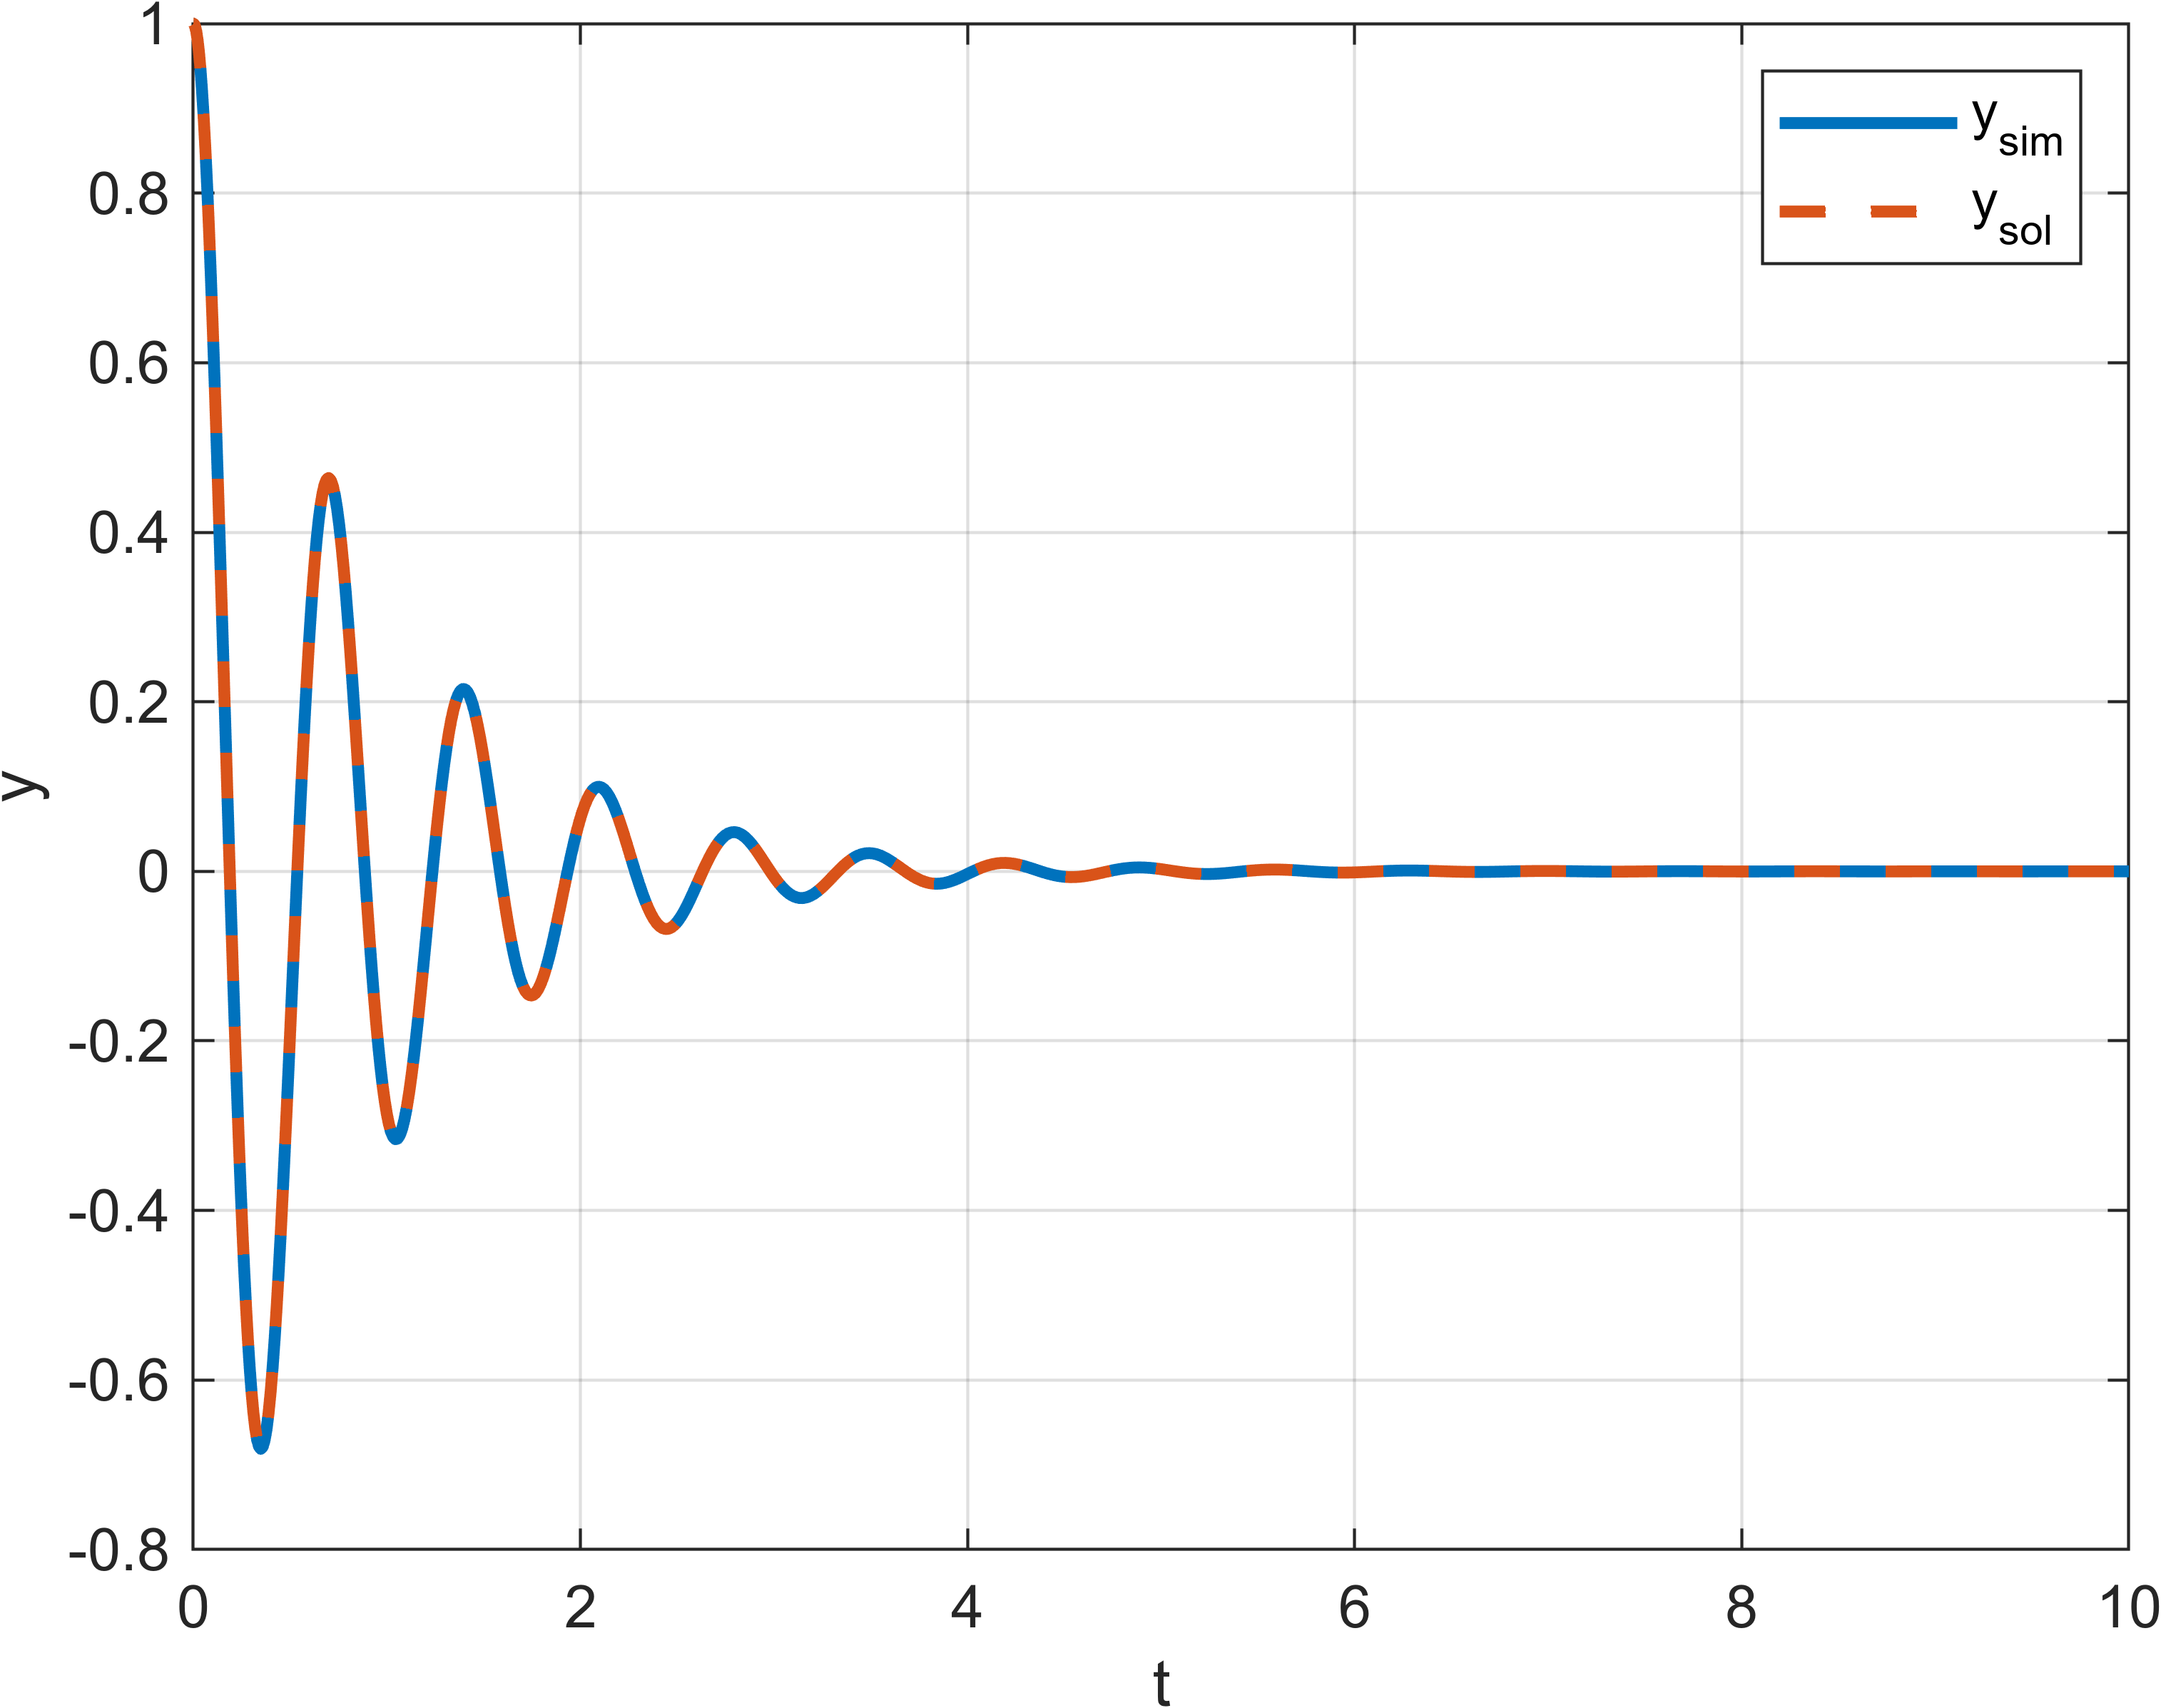
\includegraphics[width=1\textwidth, trim={0cm 0cm 0cm 0cm}]{../images/1_2.png}
    \caption{Эксперимент 2}
    \label{fig:exp2}
\end{figure}

Графики снова совпадают. Также можно заметить, что система асимптотически устойчива, так как все корни имеют отрицательные вещественные части.
\section{Эксперимент 3}
\[y(0) = 1,\, \dot y(0) = 0 \quad \lambda_1 = j9,\, \lambda_2 = -j9\]

Также как и в прошлых экспериментах по характеристическим корням построим исходное уравнение:
\[(\lambda - \lambda_1)(\lambda - \lambda_2) = (\lambda - j9)(\lambda + j9) = \lambda^2 + 81 = 0\]

Отсюда $a_0 = 81$, $a_1 = 0$. Теперь по характеристическим корням найдем выражение свободной составляющей движения в общем виде:
\[y_{\text{св}}(t) = C_1 sin(9t) + C_2 cos(9t)\]

Найдем производную:
\[\dot y_{\text{св}}(t) = 9C_1 cos(9t) - 9C_2 sin(9t)\]

Подставим начальные условия:
\[y_{\text{св}}(0) = C_2 = 1\]
\[\dot y_{\text{св}}(0) = 9C_1 = 0\]
\[C_1 = 0\]

\[y_{\text{св}}(t) = cos(9t)\]

Сравним результаты моделирования и аналитического решения:
\begin{figure}[H]
    \centering
    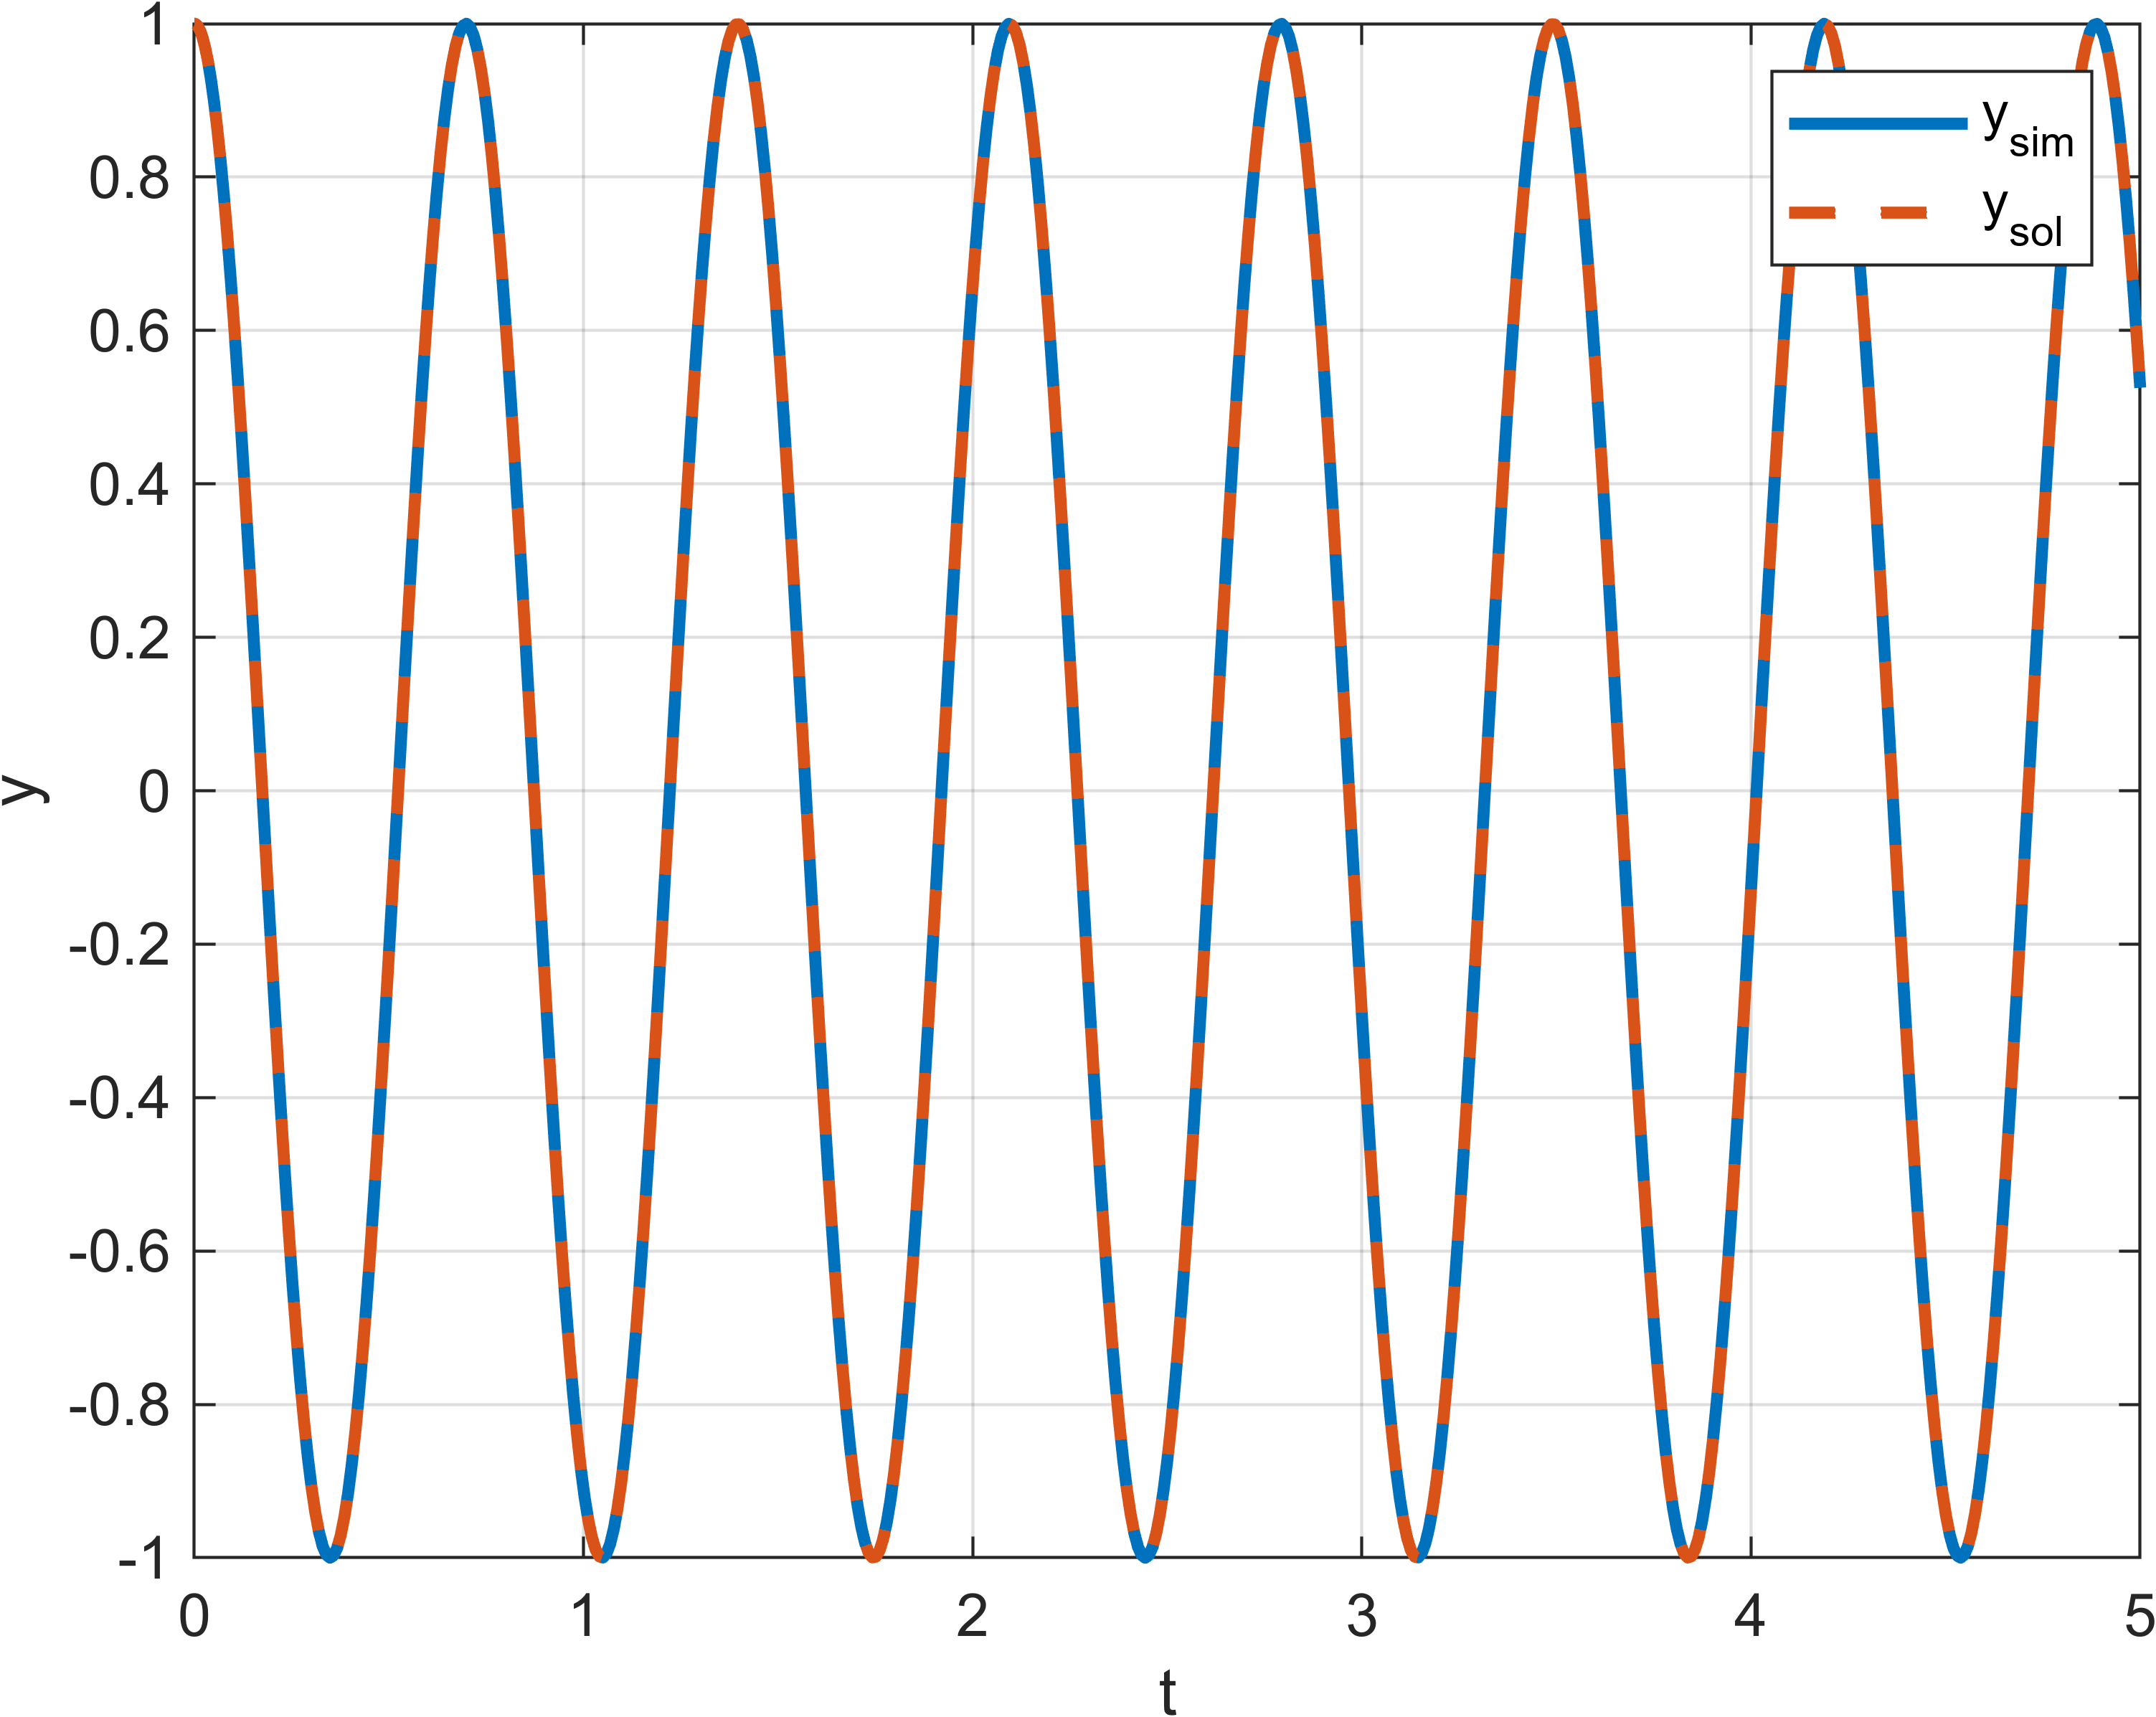
\includegraphics[width=1\textwidth, trim={0cm 0cm 0cm 0cm}]{../images/1_3.png}
    \caption{Эксперимент 3}
    \label{fig:exp3}
\end{figure}

Графики снова совпадают. В этот раз система находится на границе устойчивости, так как корни имеют нулевую вещественную часть.
\section{Эксперимент 4}
\[y(0) = 0.05,\, \dot y(0) = 0 \quad \lambda_1 = 1.1 + j9,\, \lambda_2 = 1.1 - j9\]

Также как и в прошлых экспериментах по характеристическим корням построим исходное уравнение:
\[(\lambda - \lambda_1)(\lambda - \lambda_2) = (\lambda - 1.1 - j9)(\lambda - 1.1 + j9) = \lambda^2 - 2.2\lambda + 82.21 = 0\]

Отсюда $a_0 = 82.21$, $a_1 = -2.2$. Теперь по характеристическим корням найдем выражение свободной составляющей движения в общем виде:
\[y_{\text{св}}(t) = C_1 e^{1.1 t} sin(9t) + C_2 e^{1.1 t} cos(9t)\]

Найдем производную:
\[\dot y_{\text{св}}(t) = 1.1C_1 e^{1.1 t} sin(9t) + 9C_1 e^{1.1 t} cos(9t) + 1.1C_2 e^{1.1 t} cos(9t) - 9C_2 e^{1.1 t} sin(9t)\]

Подставим начальные условия:
\[y_{\text{св}}(0) = C_2 = 0.05\]
\[\dot y_{\text{св}}(0) = 9C_1 + 1.1C_2 = 0\]
\[C_1 = -\frac{1.1}{9} \cdot 0.05\]

\[y_{\text{св}}(t) = -\frac{1.1}{9} \cdot 0.05 e^{1.1 t} sin(9t) + 0.05 e^{1.1 t} cos(9t)\]

Сравним результаты моделирования и аналитического решения:
\begin{figure}[H]
    \centering
    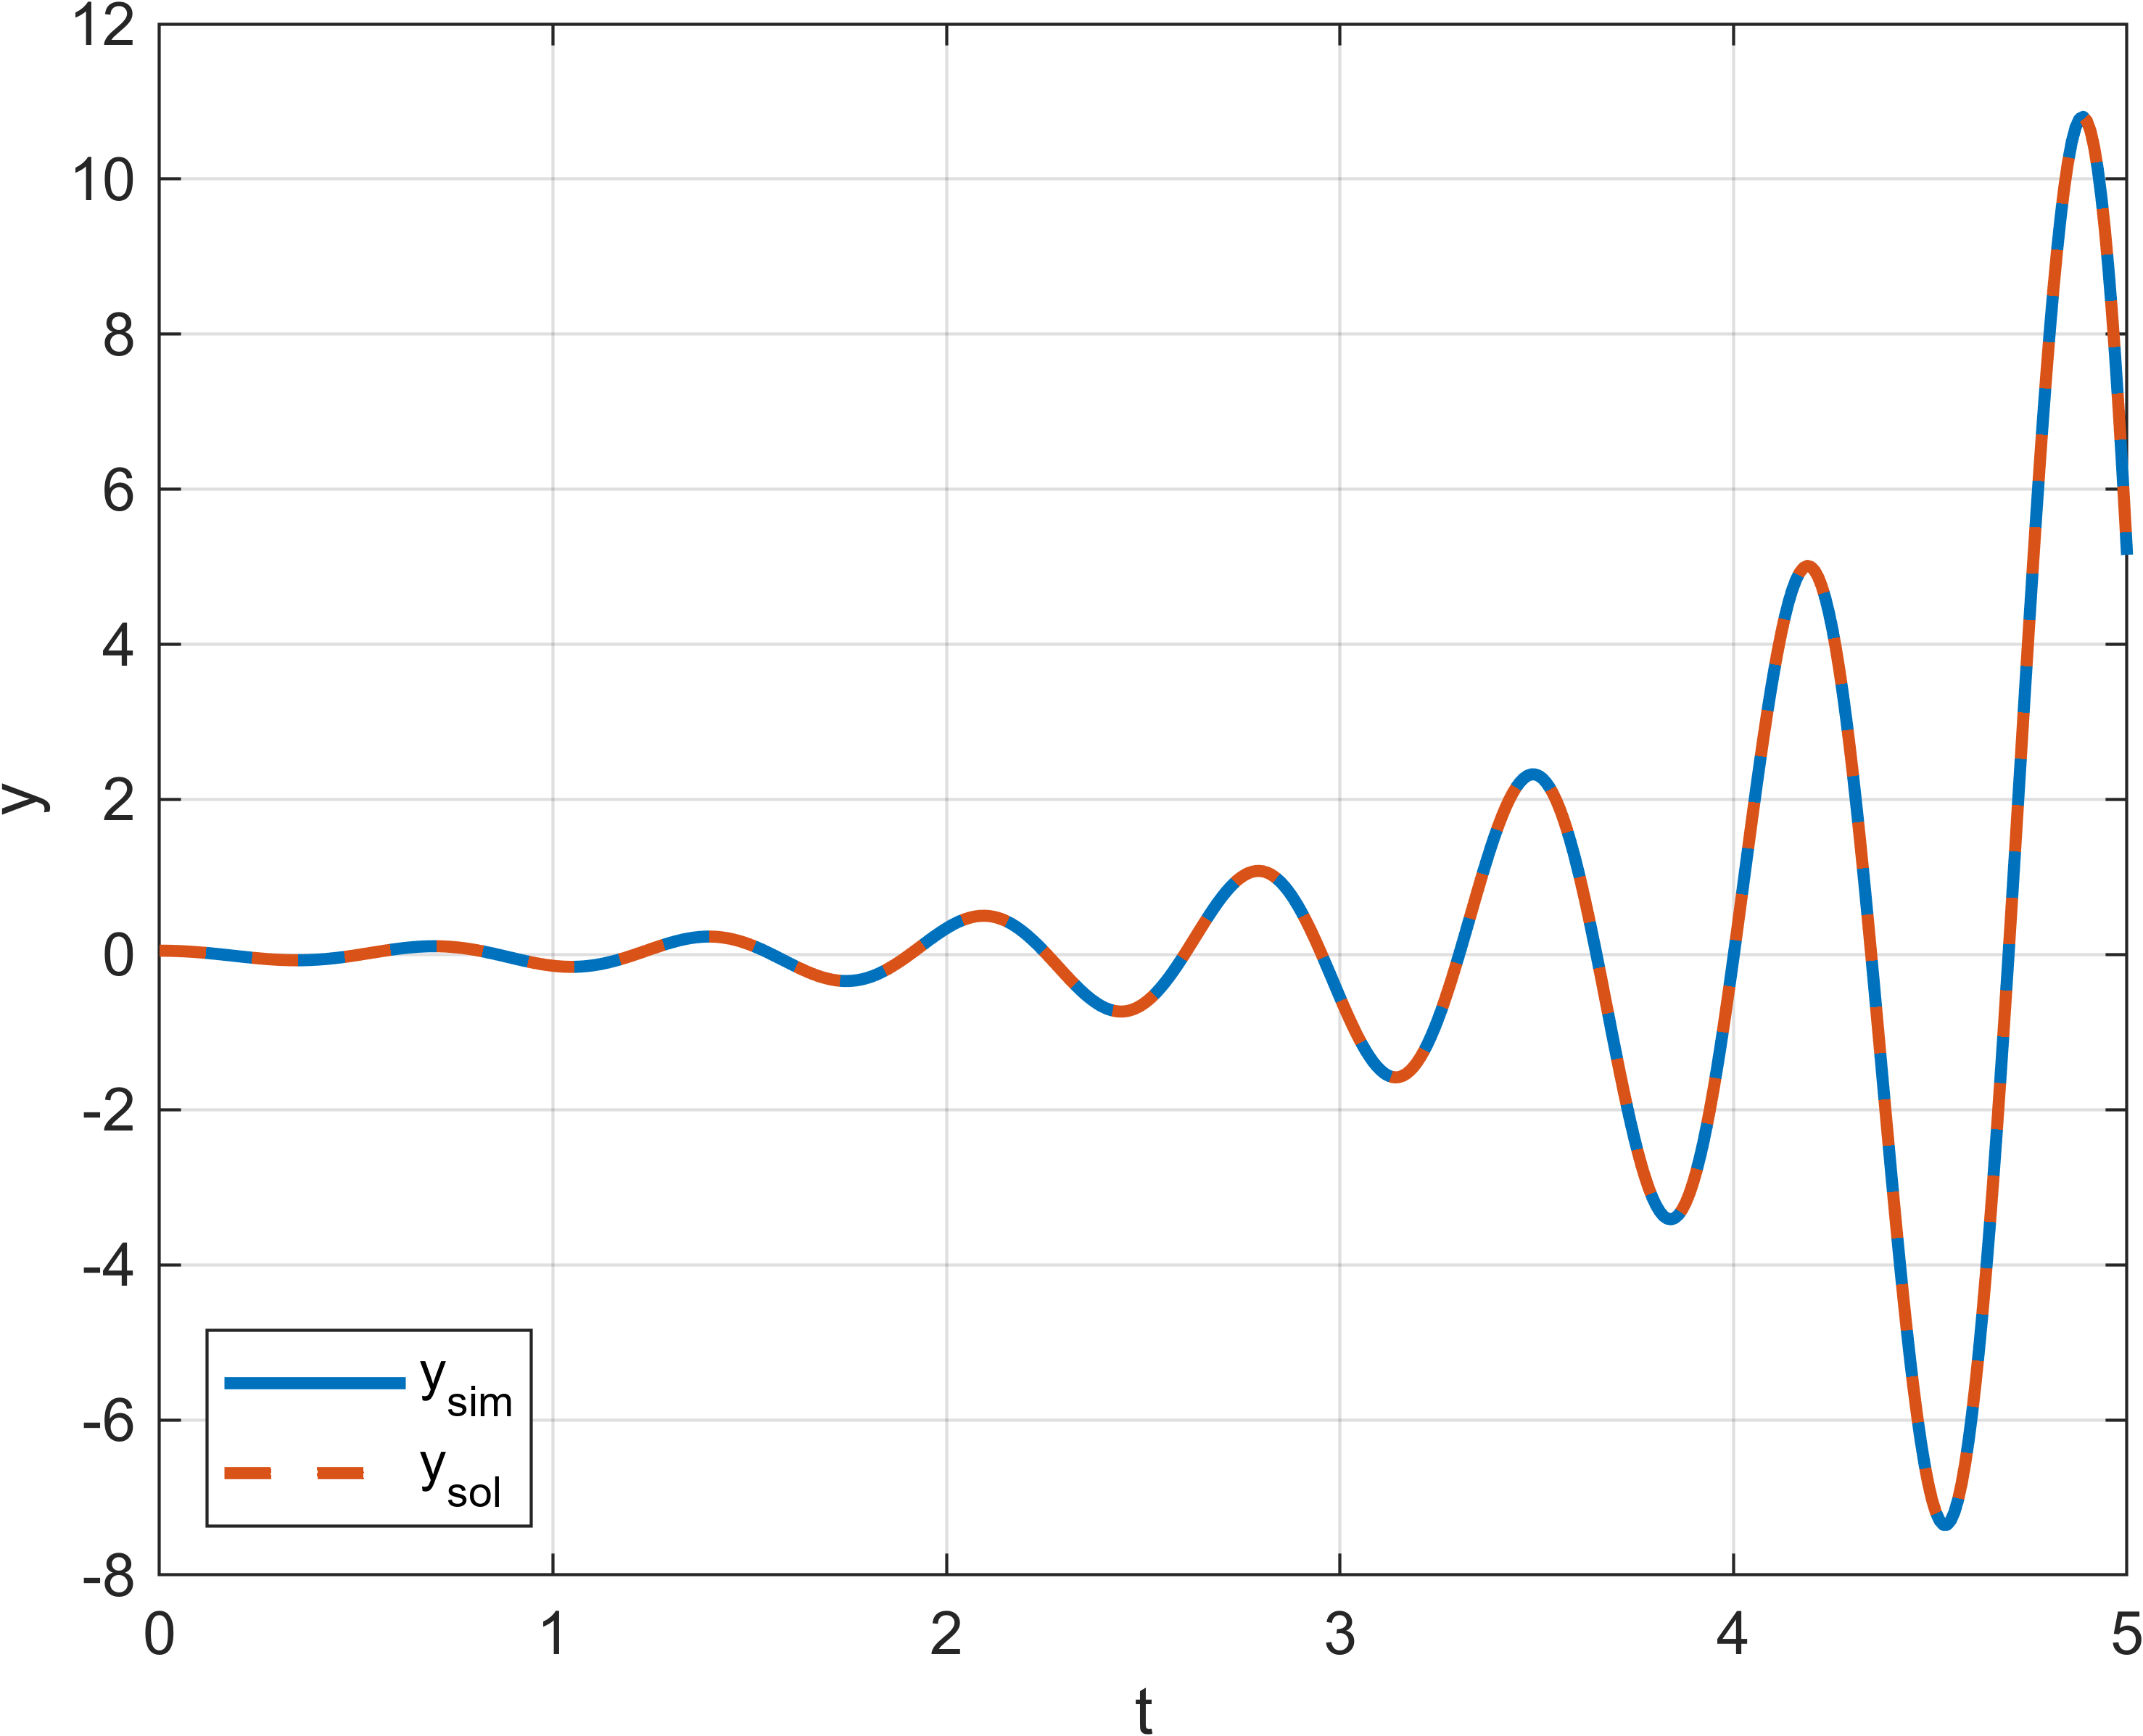
\includegraphics[width=1\textwidth, trim={0cm 0cm 0cm 0cm}]{../images/1_4.png}
    \caption{Эксперимент 4}
    \label{fig:exp4}
\end{figure}

Графики снова совпадают. Также можно заметить, что система не устойчива, так как корни имеют положительную вещественную часть.
\section{Эксперимент 5}
\[y(0) = 0.05,\, \dot y(0) = 0 \quad \lambda_1 = 3,\, \lambda_2 = 1\]

Также как и в прошлых экспериментах по характеристическим корням построим исходное уравнение:
\[(\lambda - \lambda_1)(\lambda - \lambda_2) = (\lambda - 3)(\lambda - 1) = \lambda^2 - 4\lambda + 3 = 0\]

Отсюда $a_0 = 3$, $a_1 = -4$. Теперь по характеристическим корням найдем выражение свободной составляющей движения в общем виде:
\[y_{\text{св}}(t) = C_1 e^{3 t} + C_2 e^{t}\]

Найдем производную:
\[\dot y_{\text{св}}(t) = 3C_1 e^{3 t} + C_2 e^{t}\]

Подставим начальные условия:
\[y_{\text{св}}(0) = C_1 + C_2 = 0.05\]
\[\dot y_{\text{св}}(0) = 3C_1 - C_2 = 0\]
\[C_1 = -\frac{1}{40},\, C_2 = \frac{3}{40}\]

Сравним результаты моделирования и аналитического решения:
\begin{figure}[H]
    \centering
    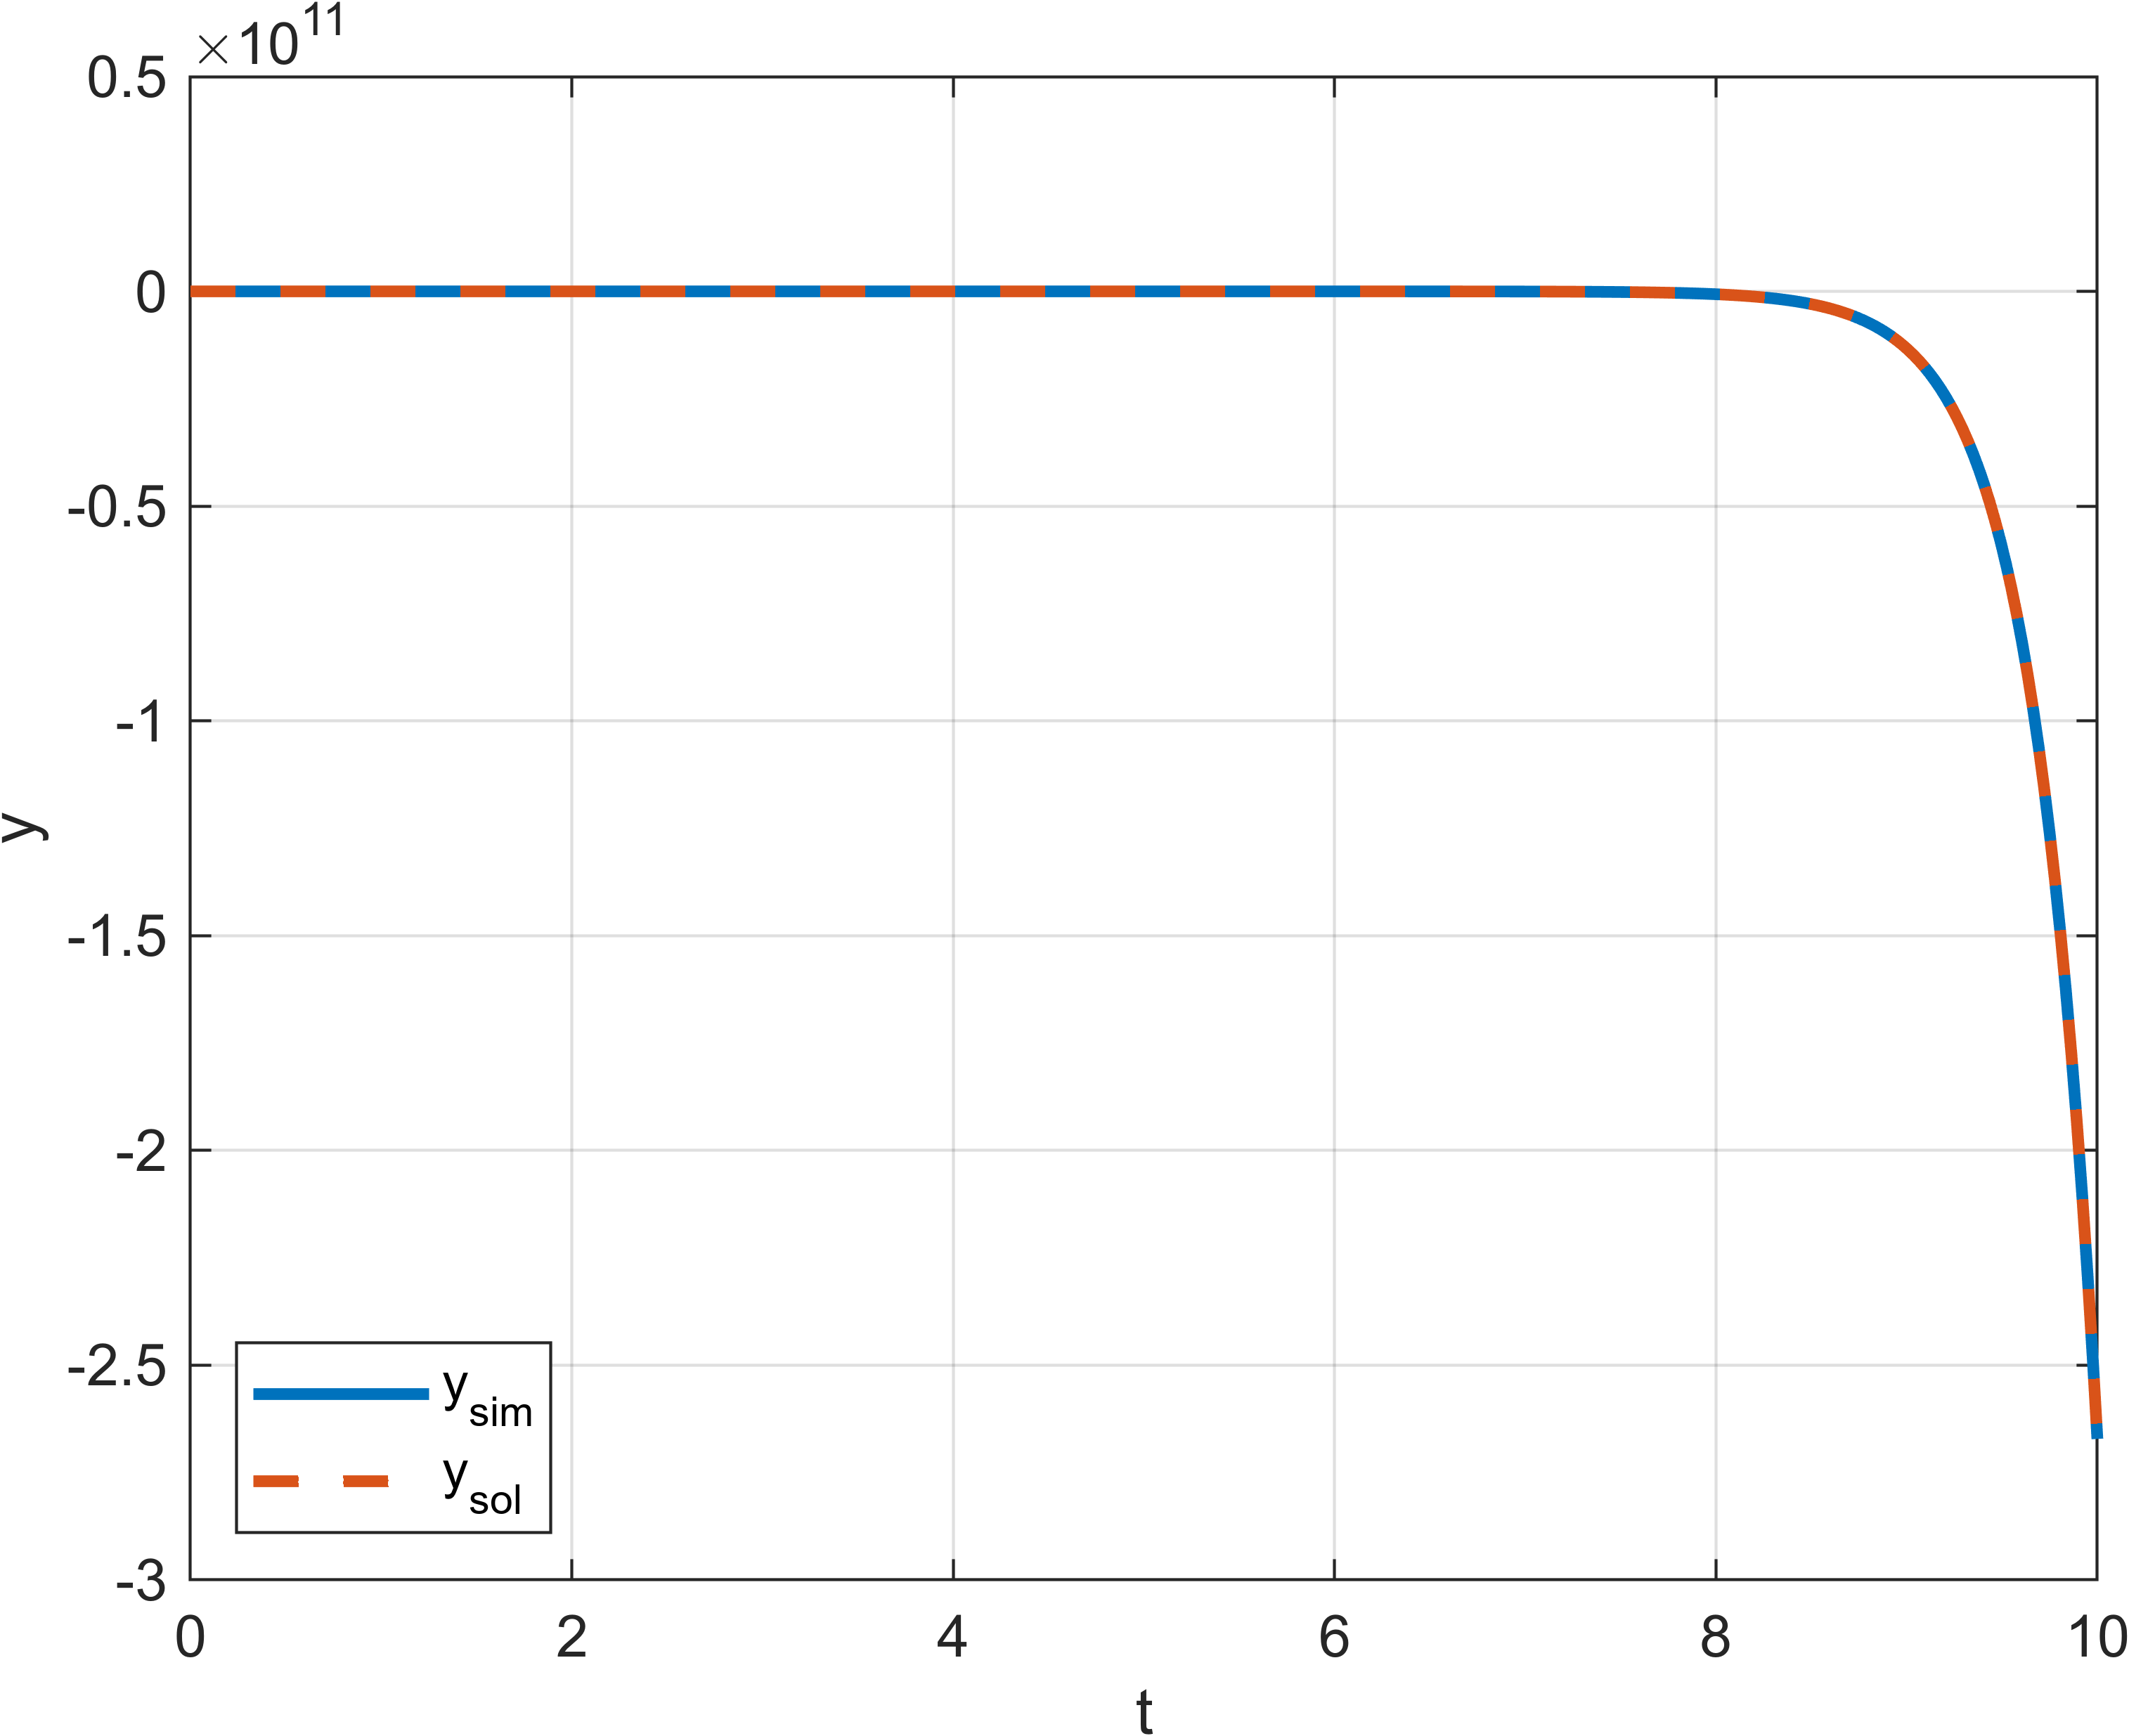
\includegraphics[width=1\textwidth, trim={0cm 0cm 0cm 0cm}]{../images/1_5.png}
    \caption{Эксперимент 5}
    \label{fig:exp5}
\end{figure}

Графики снова совпадают. Также можно заметить, что система не устойчива, так как корни имеют положительную вещественную часть.
\section{Эксперимент 6}
\[y(0) = 0,\, \dot y(0) = 0.1 \quad \lambda_1 = -0.7,\, \lambda_2 = 0.7\]

Также как и в прошлых экспериментах по характеристическим корням построим исходное уравнение:
\[(\lambda - \lambda_1)(\lambda - \lambda_2) = (\lambda + 0.7)(\lambda - 0.7) = \lambda^2 - 0.49 = 0\]

Отсюда $a_0 = -0.49$, $a_1 = 0$. Теперь по характеристическим корням найдем выражение свободной составляющей движения в общем виде:
\[y_{\text{св}}(t) = C_1 e^{-0.7 t} + C_2 e^{0.7 t}\]

Найдем производную:
\[\dot y_{\text{св}}(t) = -0.7C_1 e^{-0.7 t} + 0.7C_2 e^{0.7 t}\]

Подставим начальные условия:
\[y_{\text{св}}(0) = C_1 + C_2 = 0\]
\[\dot y_{\text{св}}(0) = -0.7C_1 + 0.7C_2 = 0.1\]
\[C_1 = -\frac{1}{14},\, C_2 = \frac{1}{14}\]
\[y_{\text{св}}(t) = -\frac{1}{14} e^{-0.7 t} + \frac{1}{14} e^{0.7 t}\]

Сравним результаты моделирования и аналитического решения:
\begin{figure}[H]
    \centering
    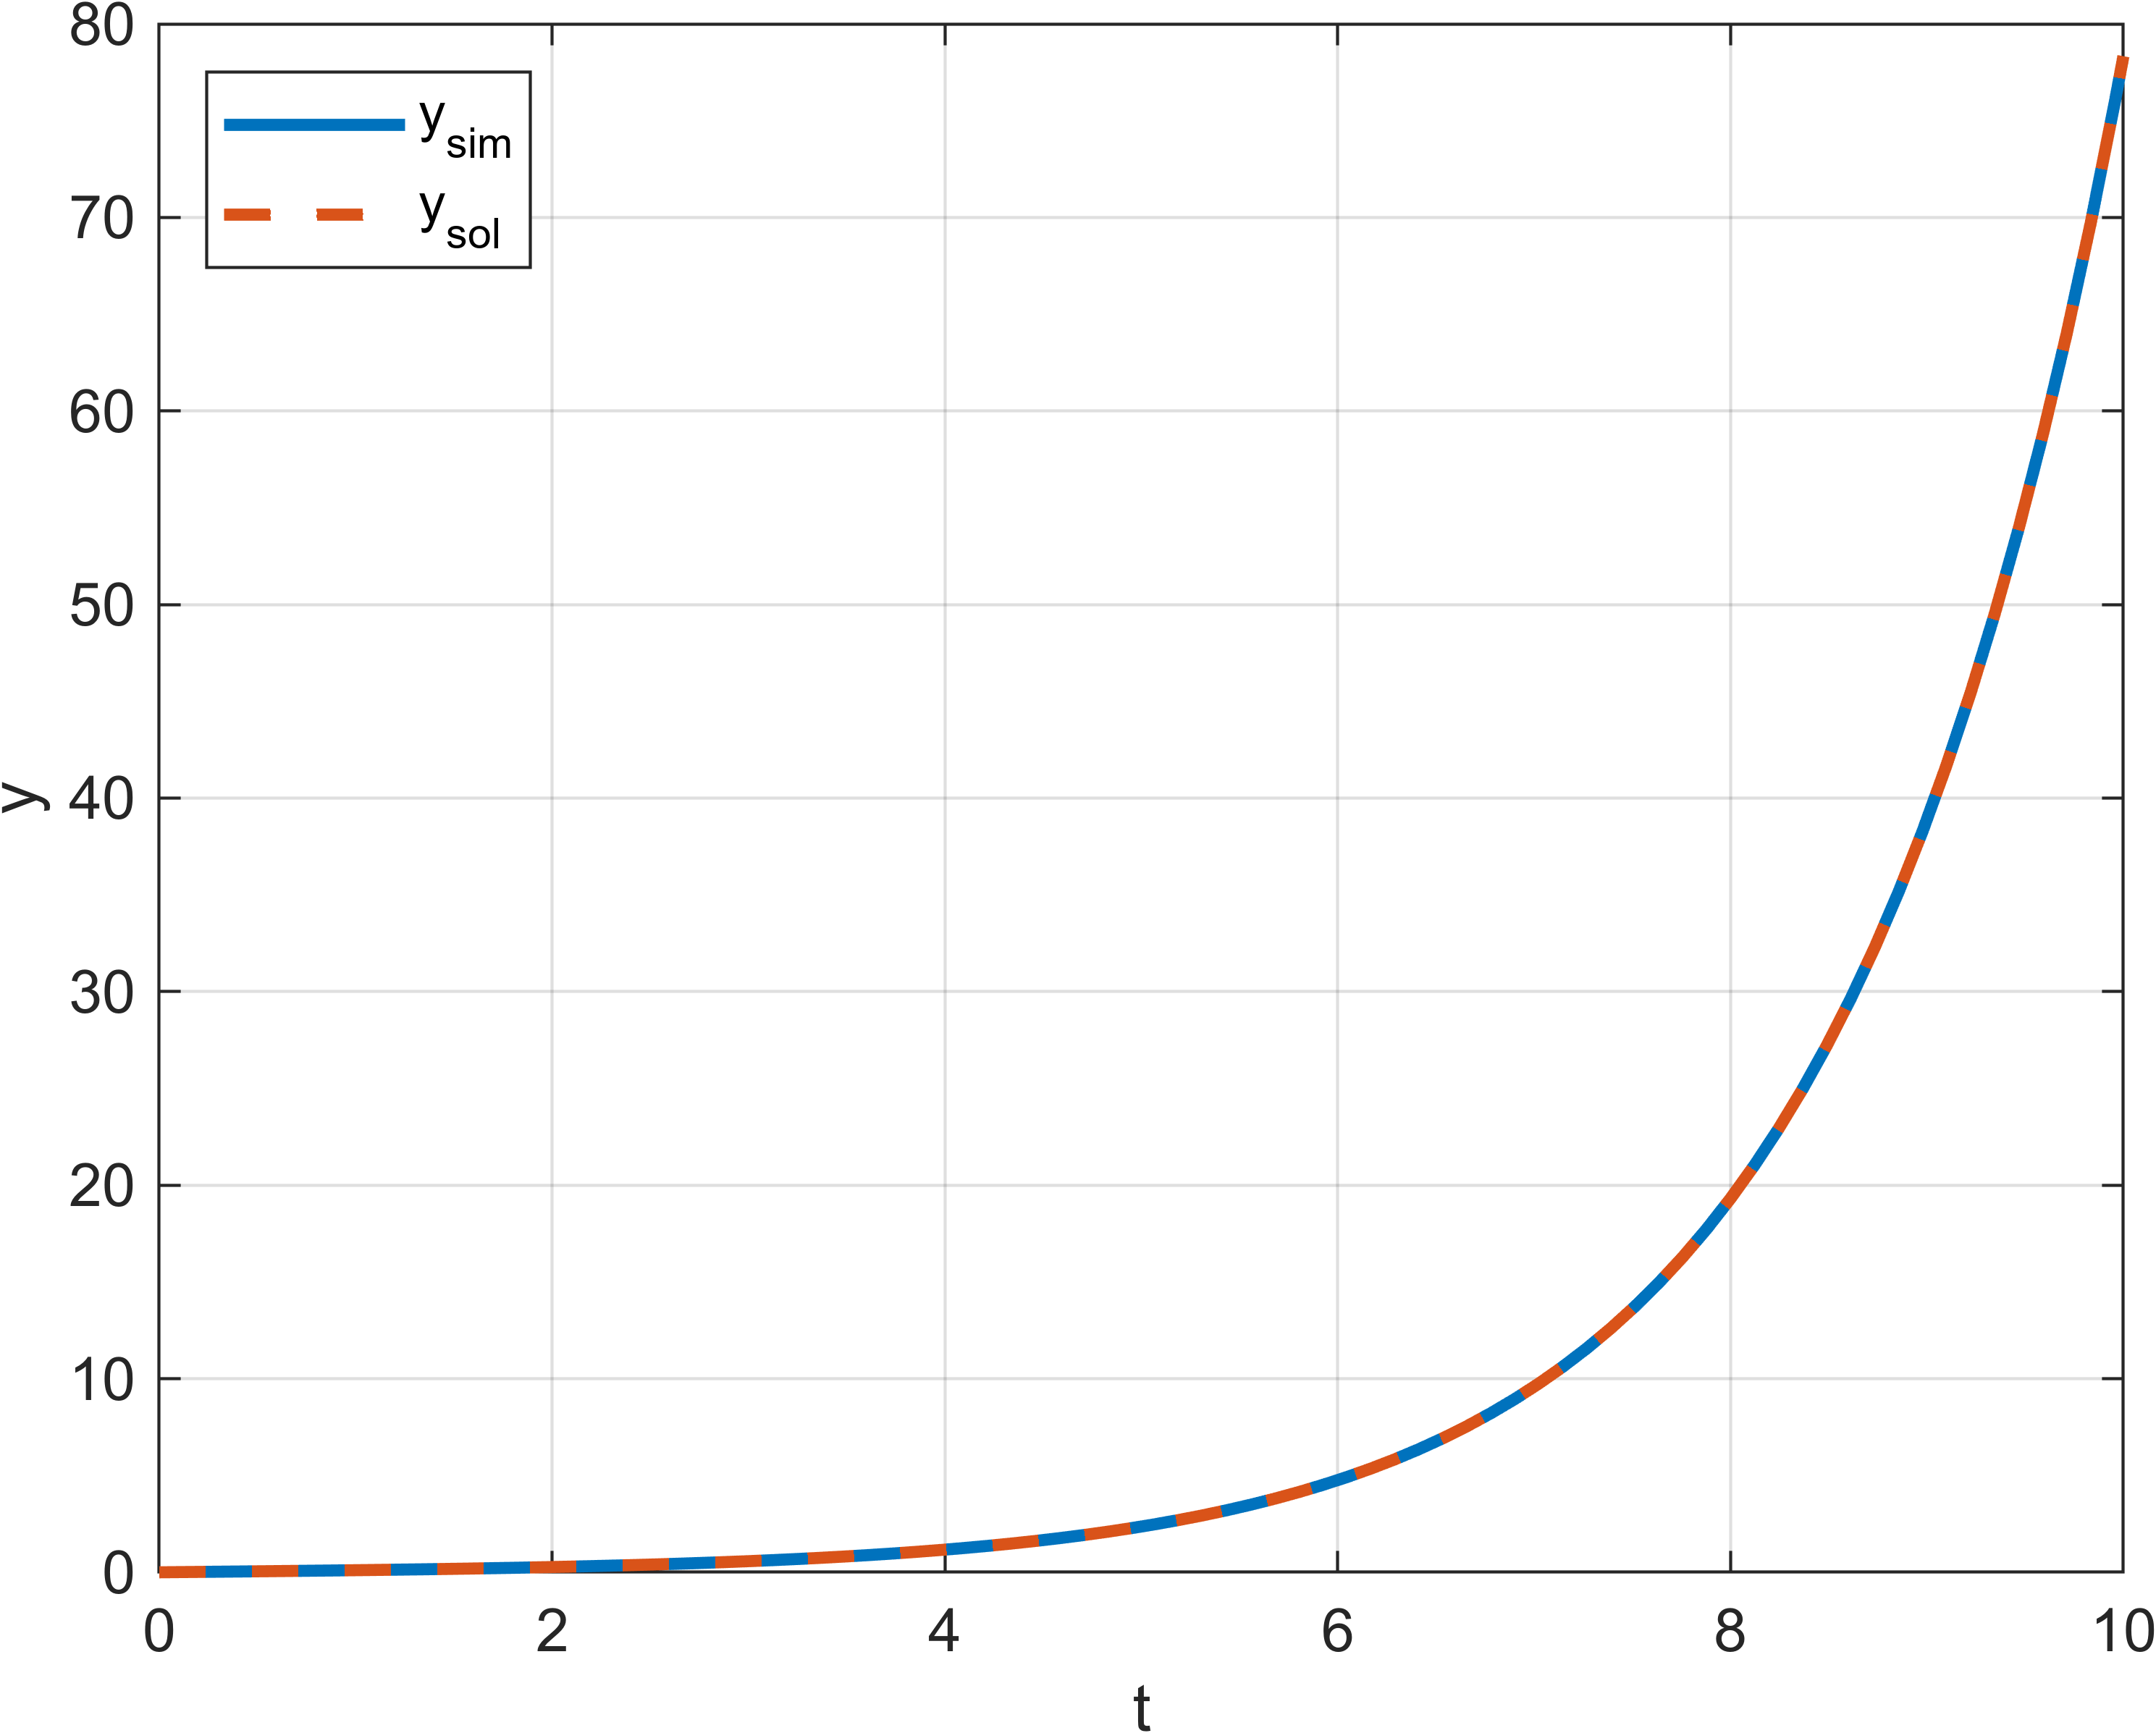
\includegraphics[width=1\textwidth, trim={0cm 0cm 0cm 0cm}]{../images/1_6.png}
    \caption{Эксперимент 6}
    \label{fig:exp6}
\end{figure}

Графики снова совпадают. Также можно заметить, что система не устойчива, так как один корень имеет положительную вещественную часть.
\endinput